% DWC resource analysis -- three LUT|FF pairs (one per width-scaling case).
% Real Vivado OOC synth (xc7z020). Paste into a document with:
%   \usepackage{pgfplots}  \pgfplotsset{compat=1.16}
%   \usepgfplotslibrary{groupplots}  \usepackage{subcaption}
% Sized for ONE column of a 2-column doc (\columnwidth); acmart styles the caption.
% For a full-width version, change 'figure' -> 'figure*' and \columnwidth -> \textwidth.
\begin{figure}[t]
\centering
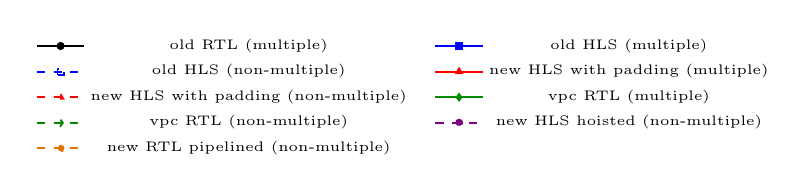
\begin{tikzpicture}
\begin{axis}[hide axis, scale only axis, width=1pt, height=1pt,
  xmin=0, xmax=1, ymin=0, ymax=1,
  legend columns=2,
  legend style={at={(0.5,0.5)}, anchor=center, draw=none, font=\tiny, /tikz/every even column/.append style={column sep=8pt}},
]
\addlegendimage{color=black,solid,mark=*, line width=0.7pt, mark size=1.1pt}
\addlegendentry{old RTL (multiple)}
\addlegendimage{color=blue,solid,mark=square*, line width=0.7pt, mark size=1.1pt}
\addlegendentry{old HLS (multiple)}
\addlegendimage{color=blue,dashed,mark=square, line width=0.7pt, mark size=1.1pt}
\addlegendentry{old HLS (non-multiple)}
\addlegendimage{color=red,solid,mark=triangle*, line width=0.7pt, mark size=1.1pt}
\addlegendentry{new HLS with padding (multiple)}
\addlegendimage{color=red,dashed,mark=triangle, line width=0.7pt, mark size=1.1pt}
\addlegendentry{new HLS with padding (non-multiple)}
\addlegendimage{color=green!55!black,solid,mark=diamond*, line width=0.7pt, mark size=1.1pt}
\addlegendentry{vpc RTL (multiple)}
\addlegendimage{color=green!55!black,dashed,mark=diamond, line width=0.7pt, mark size=1.1pt}
\addlegendentry{vpc RTL (non-multiple)}
\addlegendimage{color=violet,dashed,mark=otimes*, line width=0.7pt, mark size=1.1pt}
\addlegendentry{new HLS hoisted (non-multiple)}
\addlegendimage{color=orange!90!black,dashed,mark=pentagon*, line width=0.7pt, mark size=1.1pt}
\addlegendentry{new RTL pipelined (non-multiple)}
\end{axis}
\end{tikzpicture}
\par\medskip
\begin{subfigure}{\columnwidth}
\centering
\begin{tikzpicture}
\begin{groupplot}[
  group style={group size=2 by 1, horizontal sep=0.9cm},
  width=2.9cm, height=2.2cm, scale only axis,
  xlabel={input width (bits)},
  label style={font=\tiny}, ylabel style={yshift=-1pt},
  grid=both, ymin=0, ymax=6000, tick label style={font=\tiny},
  scaled y ticks=false, ytick={0,2000,4000,6000}, yticklabels={0,2k,4k,6k},
  legend style={font=\tiny, inner sep=1pt, row sep=-2.5pt, column sep=3pt, draw=none, fill=white, fill opacity=0.7, text opacity=1},
  every axis plot/.append style={line width=0.6pt, mark size=1.0pt},
]
\nextgroupplot[ylabel={LUTs}]
\addplot[color=black,solid,mark=*] coordinates {(20,16) (100,59) (300,308) (500,507) (750,759) (1000,1008)};
\addplot[color=blue,solid,mark=square*] coordinates {(20,99) (100,182) (300,389) (500,585) (750,836) (1000,1086)};
\addplot[color=blue,dashed,mark=square] coordinates {(25,241) (105,442) (305,944) (505,1466) (755,2101) (1005,2696)};
\addplot[color=red,solid,mark=triangle*] coordinates {(20,60) (100,151) (300,360) (500,559) (750,816) (1000,1071)};
\addplot[color=red,dashed,mark=triangle] coordinates {(25,115) (105,291) (305,703) (505,1113) (755,1668) (1005,2189)};
\addplot[color=green!55!black,solid,mark=diamond*] coordinates {(20,44) (100,543) (300,3300) (500,8321) (750,17073) (1000,31440)};
\addplot[color=green!55!black,dashed,mark=diamond] coordinates {(25,107) (105,1148) (305,6802) (505,16789) (755,33594) (1005,61678)};
\addplot[color=violet,dashed,mark=otimes*] coordinates {(25,144) (105,324) (305,747) (505,1162) (755,2422) (1005,3185)};
\addplot[color=orange!90!black,dashed,mark=pentagon*] coordinates {(25,101) (105,256) (305,676) (505,1092) (755,1596) (1005,2075)};
\nextgroupplot[ylabel={FFs}]
\addplot[color=black,solid,mark=*] coordinates {(20,44) (100,127) (300,331) (500,529) (750,780) (1000,1030)};
\addplot[color=blue,solid,mark=square*] coordinates {(20,140) (100,462) (300,1265) (500,2067) (750,3070) (1000,4072)};
\addplot[color=blue,dashed,mark=square] coordinates {(25,361) (105,1164) (305,3167) (505,5184) (755,7695) (1005,10166)};
\addplot[color=red,solid,mark=triangle*] coordinates {(20,115) (100,443) (300,1248) (500,2052) (750,3057) (1000,4059)};
\addplot[color=red,dashed,mark=triangle] coordinates {(25,138) (105,385) (305,992) (505,1599) (755,2350) (1005,3105)};
\addplot[color=green!55!black,solid,mark=diamond*] coordinates {(20,39) (100,126) (300,329) (500,532) (750,785) (1000,1035)};
\addplot[color=green!55!black,dashed,mark=diamond] coordinates {(25,49) (105,155) (305,338) (505,547) (755,814) (1005,1066)};
\addplot[color=violet,dashed,mark=otimes*] coordinates {(25,140) (105,385) (305,992) (505,1599) (755,2351) (1005,3105)};
\addplot[color=orange!90!black,dashed,mark=pentagon*] coordinates {(25,77) (105,240) (305,641) (505,1043) (755,1559) (1005,2047)};
\end{groupplot}
\end{tikzpicture}
\caption{Increasing input width (output fixed at 10). Left: LUTs, right: FFs. vpc (downscale) leaves the frame: its per-lane placement crossbar grows linearly with input width (up to 31k/62k LUT at 1000/1005 in; see analysis).}
\end{subfigure}
\par\medskip
\begin{subfigure}{\columnwidth}
\centering
\begin{tikzpicture}
\begin{groupplot}[
  group style={group size=2 by 1, horizontal sep=0.9cm},
  width=2.9cm, height=2.2cm, scale only axis,
  xlabel={output width (bits)},
  label style={font=\tiny}, ylabel style={yshift=-1pt},
  grid=both, ymin=0, ymax=6000, tick label style={font=\tiny},
  scaled y ticks=false, ytick={0,2000,4000,6000}, yticklabels={0,2k,4k,6k},
  legend style={font=\tiny, inner sep=1pt, row sep=-2.5pt, column sep=3pt, draw=none, fill=white, fill opacity=0.7, text opacity=1},
  every axis plot/.append style={line width=0.6pt, mark size=1.0pt},
]
\nextgroupplot[ylabel={LUTs}]
\addplot[color=black,solid,mark=*] coordinates {(20,9) (100,13) (300,15) (500,16) (750,17) (1000,16)};
\addplot[color=blue,solid,mark=square*] coordinates {(20,114) (100,157) (300,259) (500,360) (750,482) (1000,610)};
\addplot[color=blue,dashed,mark=square] coordinates {(25,240) (105,451) (305,955) (505,1452) (755,2079) (1005,2708)};
\addplot[color=red,solid,mark=triangle*] coordinates {(20,42) (100,85) (300,189) (500,296) (750,425) (1000,550)};
\addplot[color=red,dashed,mark=triangle] coordinates {(25,123) (105,261) (305,602) (505,970) (755,1323) (1005,1691)};
\addplot[color=green!55!black,solid,mark=diamond*] coordinates {(20,26) (100,50) (300,74) (500,116) (750,155) (1000,174)};
\addplot[color=green!55!black,dashed,mark=diamond] coordinates {(25,54) (105,160) (305,417) (505,625) (755,1035) (1005,980)};
\addplot[color=violet,dashed,mark=otimes*] coordinates {(25,152) (105,345) (305,813) (505,1296) (755,1778) (1005,2258)};
\addplot[color=orange!90!black,dashed,mark=pentagon*] coordinates {(25,87) (105,324) (305,787) (505,1217) (755,1710) (1005,2226)};
\nextgroupplot[ylabel={FFs}]
\addplot[color=black,solid,mark=*] coordinates {(20,33) (100,116) (300,317) (500,518) (750,769) (1000,1019)};
\addplot[color=blue,solid,mark=square*] coordinates {(20,131) (100,373) (300,974) (500,1575) (750,2326) (1000,3076)};
\addplot[color=blue,dashed,mark=square] coordinates {(25,346) (105,1069) (305,2872) (505,4675) (755,6928) (1005,9181)};
\addplot[color=red,solid,mark=triangle*] coordinates {(20,100) (100,345) (300,947) (500,1549) (750,2301) (1000,3051)};
\addplot[color=red,dashed,mark=triangle] coordinates {(25,156) (105,482) (305,1285) (505,2088) (755,3091) (1005,4091)};
\addplot[color=green!55!black,solid,mark=diamond*] coordinates {(20,39) (100,126) (300,329) (500,532) (750,785) (1000,1035)};
\addplot[color=green!55!black,dashed,mark=diamond] coordinates {(25,49) (105,135) (305,338) (505,541) (755,794) (1005,1044)};
\addplot[color=violet,dashed,mark=otimes*] coordinates {(25,157) (105,486) (305,1292) (505,2089) (755,3096) (1005,4100)};
\addplot[color=orange!90!black,dashed,mark=pentagon*] coordinates {(25,80) (105,243) (305,649) (505,1049) (755,1558) (1005,2052)};
\end{groupplot}
\end{tikzpicture}
\caption{Increasing output width (input fixed at 10). Left: LUTs, right: FFs.}
\end{subfigure}
\par\medskip
\begin{subfigure}{\columnwidth}
\centering
\begin{tikzpicture}
\begin{groupplot}[
  group style={group size=2 by 1, horizontal sep=0.9cm},
  width=2.9cm, height=2.2cm, scale only axis,
  xlabel={input+output (bits)},
  label style={font=\tiny}, ylabel style={yshift=-1pt},
  grid=both, ymin=0, ymax=6000, tick label style={font=\tiny},
  scaled y ticks=false, ytick={0,2000,4000,6000}, yticklabels={0,2k,4k,6k},
  legend style={font=\tiny, inner sep=1pt, row sep=-2.5pt, column sep=3pt, draw=none, fill=white, fill opacity=0.7, text opacity=1},
  every axis plot/.append style={line width=0.6pt, mark size=1.0pt},
]
\nextgroupplot[ylabel={LUTs}]
\addplot[color=black,solid,mark=*] coordinates {(96,38) (192,70) (384,134) (768,262) (1023,348)};
\addplot[color=blue,solid,mark=square*] coordinates {(96,155) (192,235) (384,395) (768,715) (1023,927)};
\addplot[color=blue,dashed,mark=square] coordinates {(92,750) (184,1340) (368,2471) (736,4767) (868,7335) (992,8357)};
\addplot[color=red,solid,mark=triangle*] coordinates {(96,115) (192,195) (384,358) (768,678) (1023,891)};
\addplot[color=red,dashed,mark=triangle] coordinates {(92,317) (184,620) (368,1237) (736,2147) (868,2701) (992,3169)};
\addplot[color=green!55!black,solid,mark=diamond*] coordinates {(96,101) (192,179) (384,342) (768,662) (1023,875)};
\addplot[color=green!55!black,dashed,mark=diamond] coordinates {(92,499) (184,890) (368,1661) (736,2723) (868,3806) (992,4339)};
\addplot[color=violet,dashed,mark=otimes*] coordinates {(92,422) (184,708) (368,1454) (736,2797) (868,3428) (992,4097)};
\addplot[color=orange!90!black,dashed,mark=pentagon*] coordinates {(92,274) (184,530) (368,1031) (736,2002) (868,4136) (992,2615)};
\nextgroupplot[ylabel={FFs}]
\addplot[color=black,solid,mark=*] coordinates {(96,132) (192,260) (384,516) (768,1028) (1023,1368)};
\addplot[color=blue,solid,mark=square*] coordinates {(96,338) (192,626) (384,1202) (768,2354) (1023,3119)};
\addplot[color=blue,dashed,mark=square] coordinates {(92,2352) (184,4616) (368,9096) (736,18088) (868,28273) (992,32297)};
\addplot[color=red,solid,mark=triangle*] coordinates {(96,313) (192,601) (384,1177) (768,2329) (1023,3094)};
\addplot[color=red,dashed,mark=triangle] coordinates {(92,359) (184,679) (368,1321) (736,2606) (868,3073) (992,3509)};
\addplot[color=green!55!black,solid,mark=diamond*] coordinates {(96,105) (192,201) (384,393) (768,777) (1023,1032)};
\addplot[color=green!55!black,dashed,mark=diamond] coordinates {(92,114) (184,212) (368,400) (736,770) (868,910) (992,1040)};
\addplot[color=violet,dashed,mark=otimes*] coordinates {(92,359) (184,681) (368,1327) (736,2608) (868,3075) (992,3517)};
\addplot[color=orange!90!black,dashed,mark=pentagon*] coordinates {(92,201) (184,376) (368,740) (736,1444) (868,1712) (992,1955)};
\end{groupplot}
\end{tikzpicture}
\caption{Increasing both widths near-equally. Left: LUTs, right: FFs.}
\end{subfigure}
\label{fig:dwc-resources}
\end{figure}
